\subsection{Utilisations des transformations}
Voici quelques exemples de transformation d'objets. La pyramide de Sierpiński est uniquement réalisée à partir de symétries et d'homotéties.
\begin{figure}[h]
    \centering
    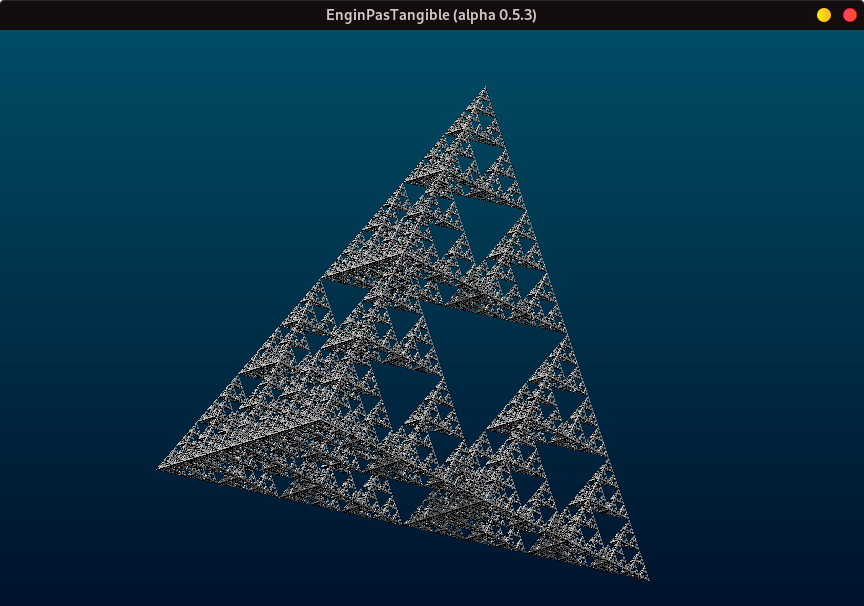
\includegraphics[width=5cm]{images/screens/sierp.png}
    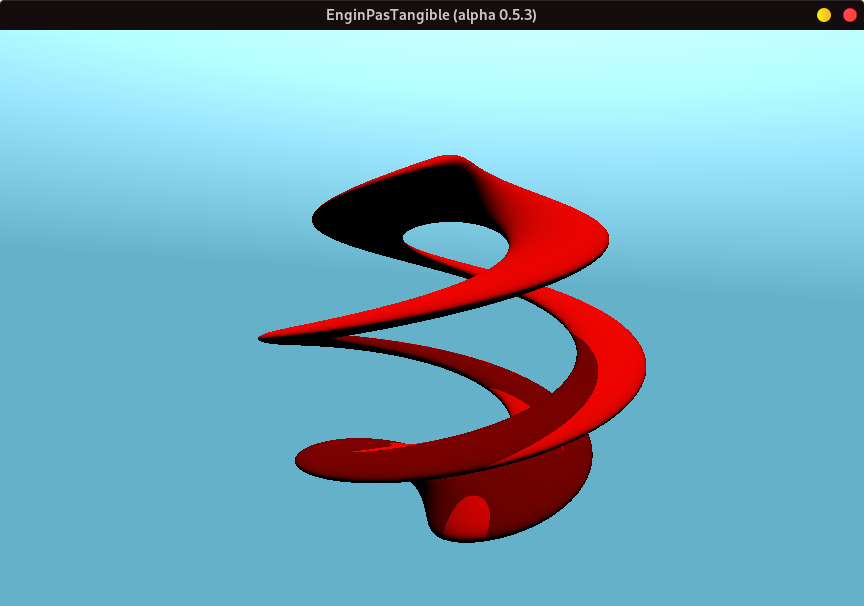
\includegraphics[width=5cm]{images/screens/modifier1.png}
    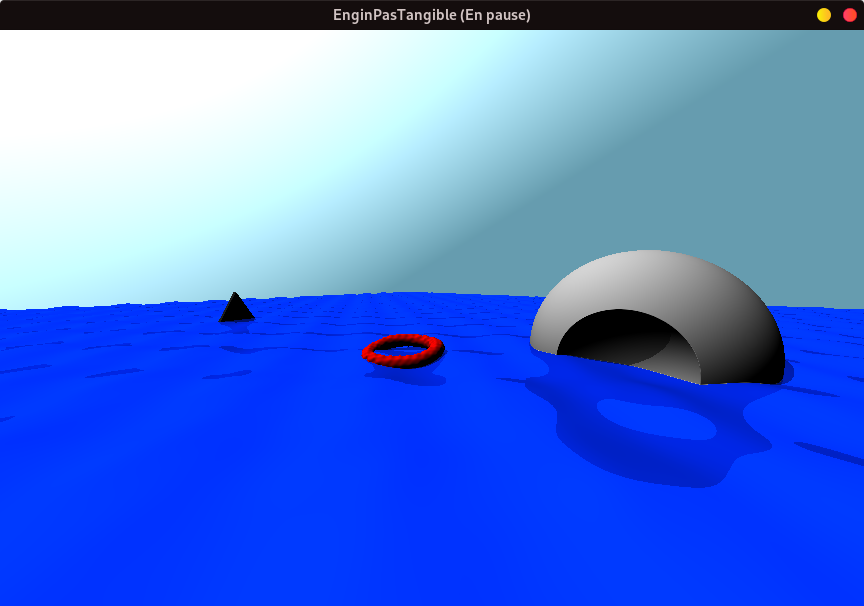
\includegraphics[width=5cm]{images/screens/modifier2.png}
    \caption{Transformations d'objets à partir de fonctions}
    \label{fig:ocean}
\end{figure}